\section{Datasets}

We tested our algorithm on Vision for Visibility Dataset (ViViD) which is released
alongside this paper. In the dataset, variations in motion and lighting are
included for testing the robustness of depth sensor and event camera.
%--------------------------------------------------------------------------%
\subsection{Sensor configuration}

To capture visual information even under various environments, three
cameras were installed along with the inertial measurement unit as in
\figref{fig:sensors}. Through this sensor system, we aim to obtain visual
information free from external lighting conditions. These unique sensor set
collects data from infrared radiation, which is dependent on the temperature of
the object, structured light depth measurement, and relative not absolute
intensity changes upon time. The dataset is provided in binary format in rosbag.
Note that in the thermal camera, the format of the image is not a typical
8-bit int but 14 bits enclosed in 16 bits.


%FIGURE
\begin{figure}[!t]
	\centering
	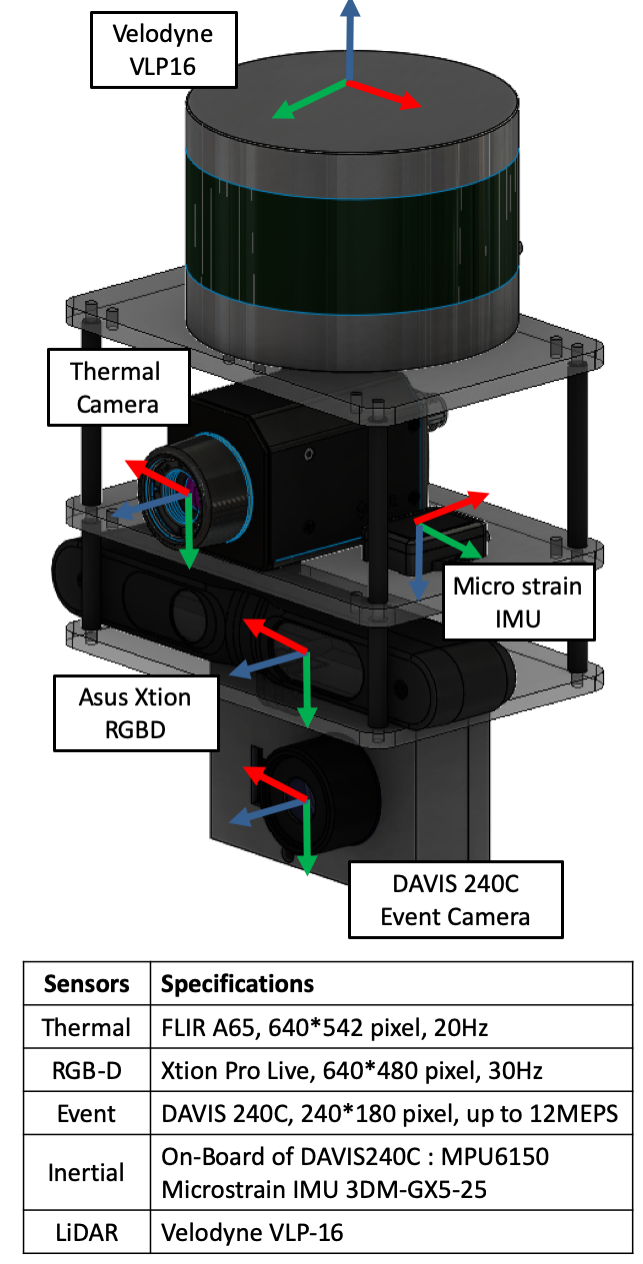
\includegraphics[width=0.7\columnwidth]{figures/sensorconfig.png}
	
	\caption{Sensors hardware configuration.}
	
	\label{fig:sensors}
	\vspace{-6mm}
\end{figure}

For calibration, we used general checkerboard and April tags for finding
extrinsic parameter between RGB-D and event camera and inertial measurement
unit. Since the DAVIS camera also produces intensity-based image, its calibration
procedure can be done for image and applied for events. However since the
thermal camera only detects differences in temperature, it does not detect
normal checkerboard pattern. We used heated printed circuit board (PCB) for
calibrating thermal camera to the system.

%--------------------------------------------------------------------------%
\subsection{Description of sequences}

The sequence list is detailed in \tabref{tab:sequences}. The sequences are
composed of two distinct locations (indoor / outdoor) and four different light
conditions (normal / dark / dimmed / varying light) with motion variances for
indoor sequences. 

%--------------------------------------------------------------------------%
\subsubsection{Environments}

The first and second batches of the dataset are recorded in different locations.
In indoor sequences, global poses of the platform are captured via motion
capture system. The scale of the room is \unit{12.3}{m} $\times$ \unit{8.9}{m}
$\times$ \unit{4.5}{m} with 12 cameras mounted on the wall for motion capture.
The system uses infrared strobes to track the reflected markers of desired
platforms. The overview of indoor sequences is provided in \figref{fig:samplesequence}.

For outdoor sequences, a pose obtained with LeGO-LOAM \cite{legoloam2018} was used
as a ground truth. The location of the outdoor trajectory is nearly enclosed by
buildings, lowering the accuracy of \ac{GPS} rather appropriate for
LiDAR-based algorithms. The total size of the enclosed region is about
\unit{60}{m} $\times$ \unit{40}{m}, and the trajectory length is around
\unit{50}{m}.

%--------------------------------------------------------------------------%
\subsubsection{Illumination and Ego-motion Variance}

In each batch, light and motion variance was applied to create disturbance.
In the real world, robots experience both uncooperative luminance and abrupt
terrain, which creates aggressive motion. The dataset consists of three
sequences from normal, dark and changing illumination conditions. For indoor
environments, rapid movements were recorded assuming drone tracking or hand-held
scenarios.

% Please add the following required packages to your document preamble:
% \usepackage{multirow}
\begin{table}[t]
	\centering
	\caption{Environment setting for each sequences}
	\begin{tabular}{ccccc}
		\hline
		Sequence                 & Ambient Light & Additional Light & Motion & Pose GT \\ \hline
		\multirow{6}{*}{Indoor}  & Bright              & OFF         & Robust & Vicon   \\ \cline{2-5} 
		& Bright              & OFF         & Fast   & Vicon   \\ \cline{2-5} 
		& Dark                & OFF         & Robust & Vicon   \\ \cline{2-5} 
		& Dark                & OFF         & Fast   & Vicon   \\ \cline{2-5} 
		& Dark                & ON          & Robust & Vicon   \\ \cline{2-5} 
		& Dark                & ON          & Fast   & Vicon   \\ \hline
		\multirow{3}{*}{Outdoor} & Bright              & OFF         & Robust & LOAM    \\ \cline{2-5} 
		& Dark                & OFF         & Robust & LOAM    \\ \cline{2-5} 
		& Dark                & ON          & Robust & LOAM    \\ \hline
	\end{tabular}
\label{tab:sequences}
\end{table}
